\chapter{Inverted Pendulum Analysis}


\section{Inverted Pendulum Description}
For this project an inverted pendulum set up is given. It consists of:
\begin{itemize}
	\item a DC motor
	\item a system of four gears linked by belt strap
	\item an arm
	\item a stick connected to the end of the arm with a liberty of movement of one degree
\end{itemize}

\begin{figure} [htbp]
	\centering
	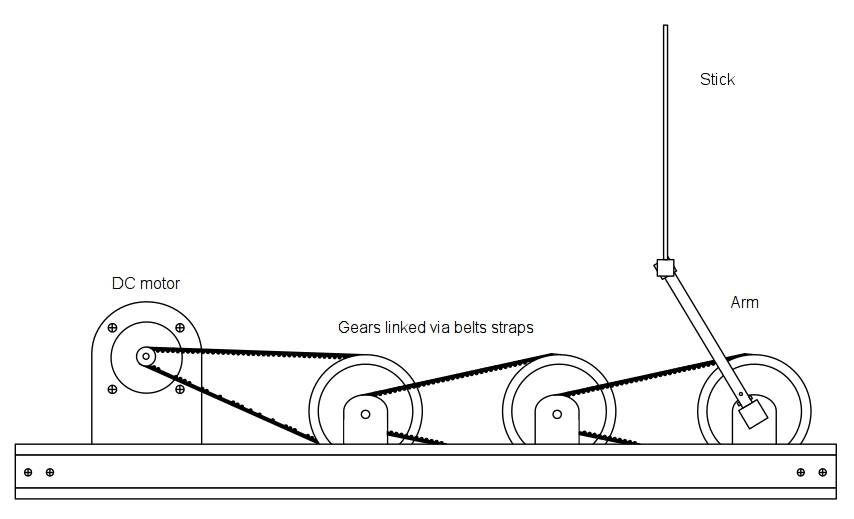
\includegraphics[width=0.8\linewidth]{figures/"Preanalysis&Requirement"/invertedPendulumDiagram}
	\caption{Diagram of the set up fully assembled} \label{fig:InvertedPendulumSetUp}
\end{figure}

\autoref{fig:InvertedPendulumSetUp} is a diagram of the set up when fully assembled. The DC motor moves the arm via the gears, a noteworthy fact is that out the four gears three are of the same size. This means that two gears do not have any influence on the torque and the angular velocity of the arm.

\section{Modelling of the Arm and Stick}\label{sec:StickArm}

%%%%%%%%%%%%% Equation template %%%%%%%%%%%%%%%
%\begin{flalign}
%\hspace{30pt} & EQUATION1 &&& \text{[UNIT]} \notag \\
%& EQUATION2 &&& \text{[UNIT]} \label{eq:LABEL} 
%\end{flalign}
%\begin{description}
%  \item[\hspace{30pt}\textnormal{where:}]\hfill \\
%  \begin{tabular}{p{30pt}lp{250pt}l}
%& $x$ & TEXT & [UNIT]  \\
%& $y$ & VERY LONG TEXT THAT IS VERY LONG AND HAS A LOT OF WORDS IN IT YET THE FORMATTING STILL LOOKS NICE AND CLEAN AND EVERYTHING IS AWESOME & [UNIT]  \\
%& $z$ & TEXT & [UNIT]
%\end{tabular}
%\end{description}
%%%%%%%%%%%%%%%%%%%%%%%%%%%%%%%%%%%%%%%%%%%%%%%
\graphicspath{{figures/Preanalysis&Requirement/PendulumModeling/}}
The goal of this section is to have a mathematical model for the behavior of the angle of the stick in relation to the angle of the arm on the motor. The angles, constants and forces used to describe the system are seen on \autoref{fig:ArmStick}.
%\todo[inline,author=Jacob]{I'd like to somehow describe the process first instead of just going along randomly and suddenly ending up with the model. "We want to achieve this so we do that" etc.}
\begin{figure}[htbp]
\centering
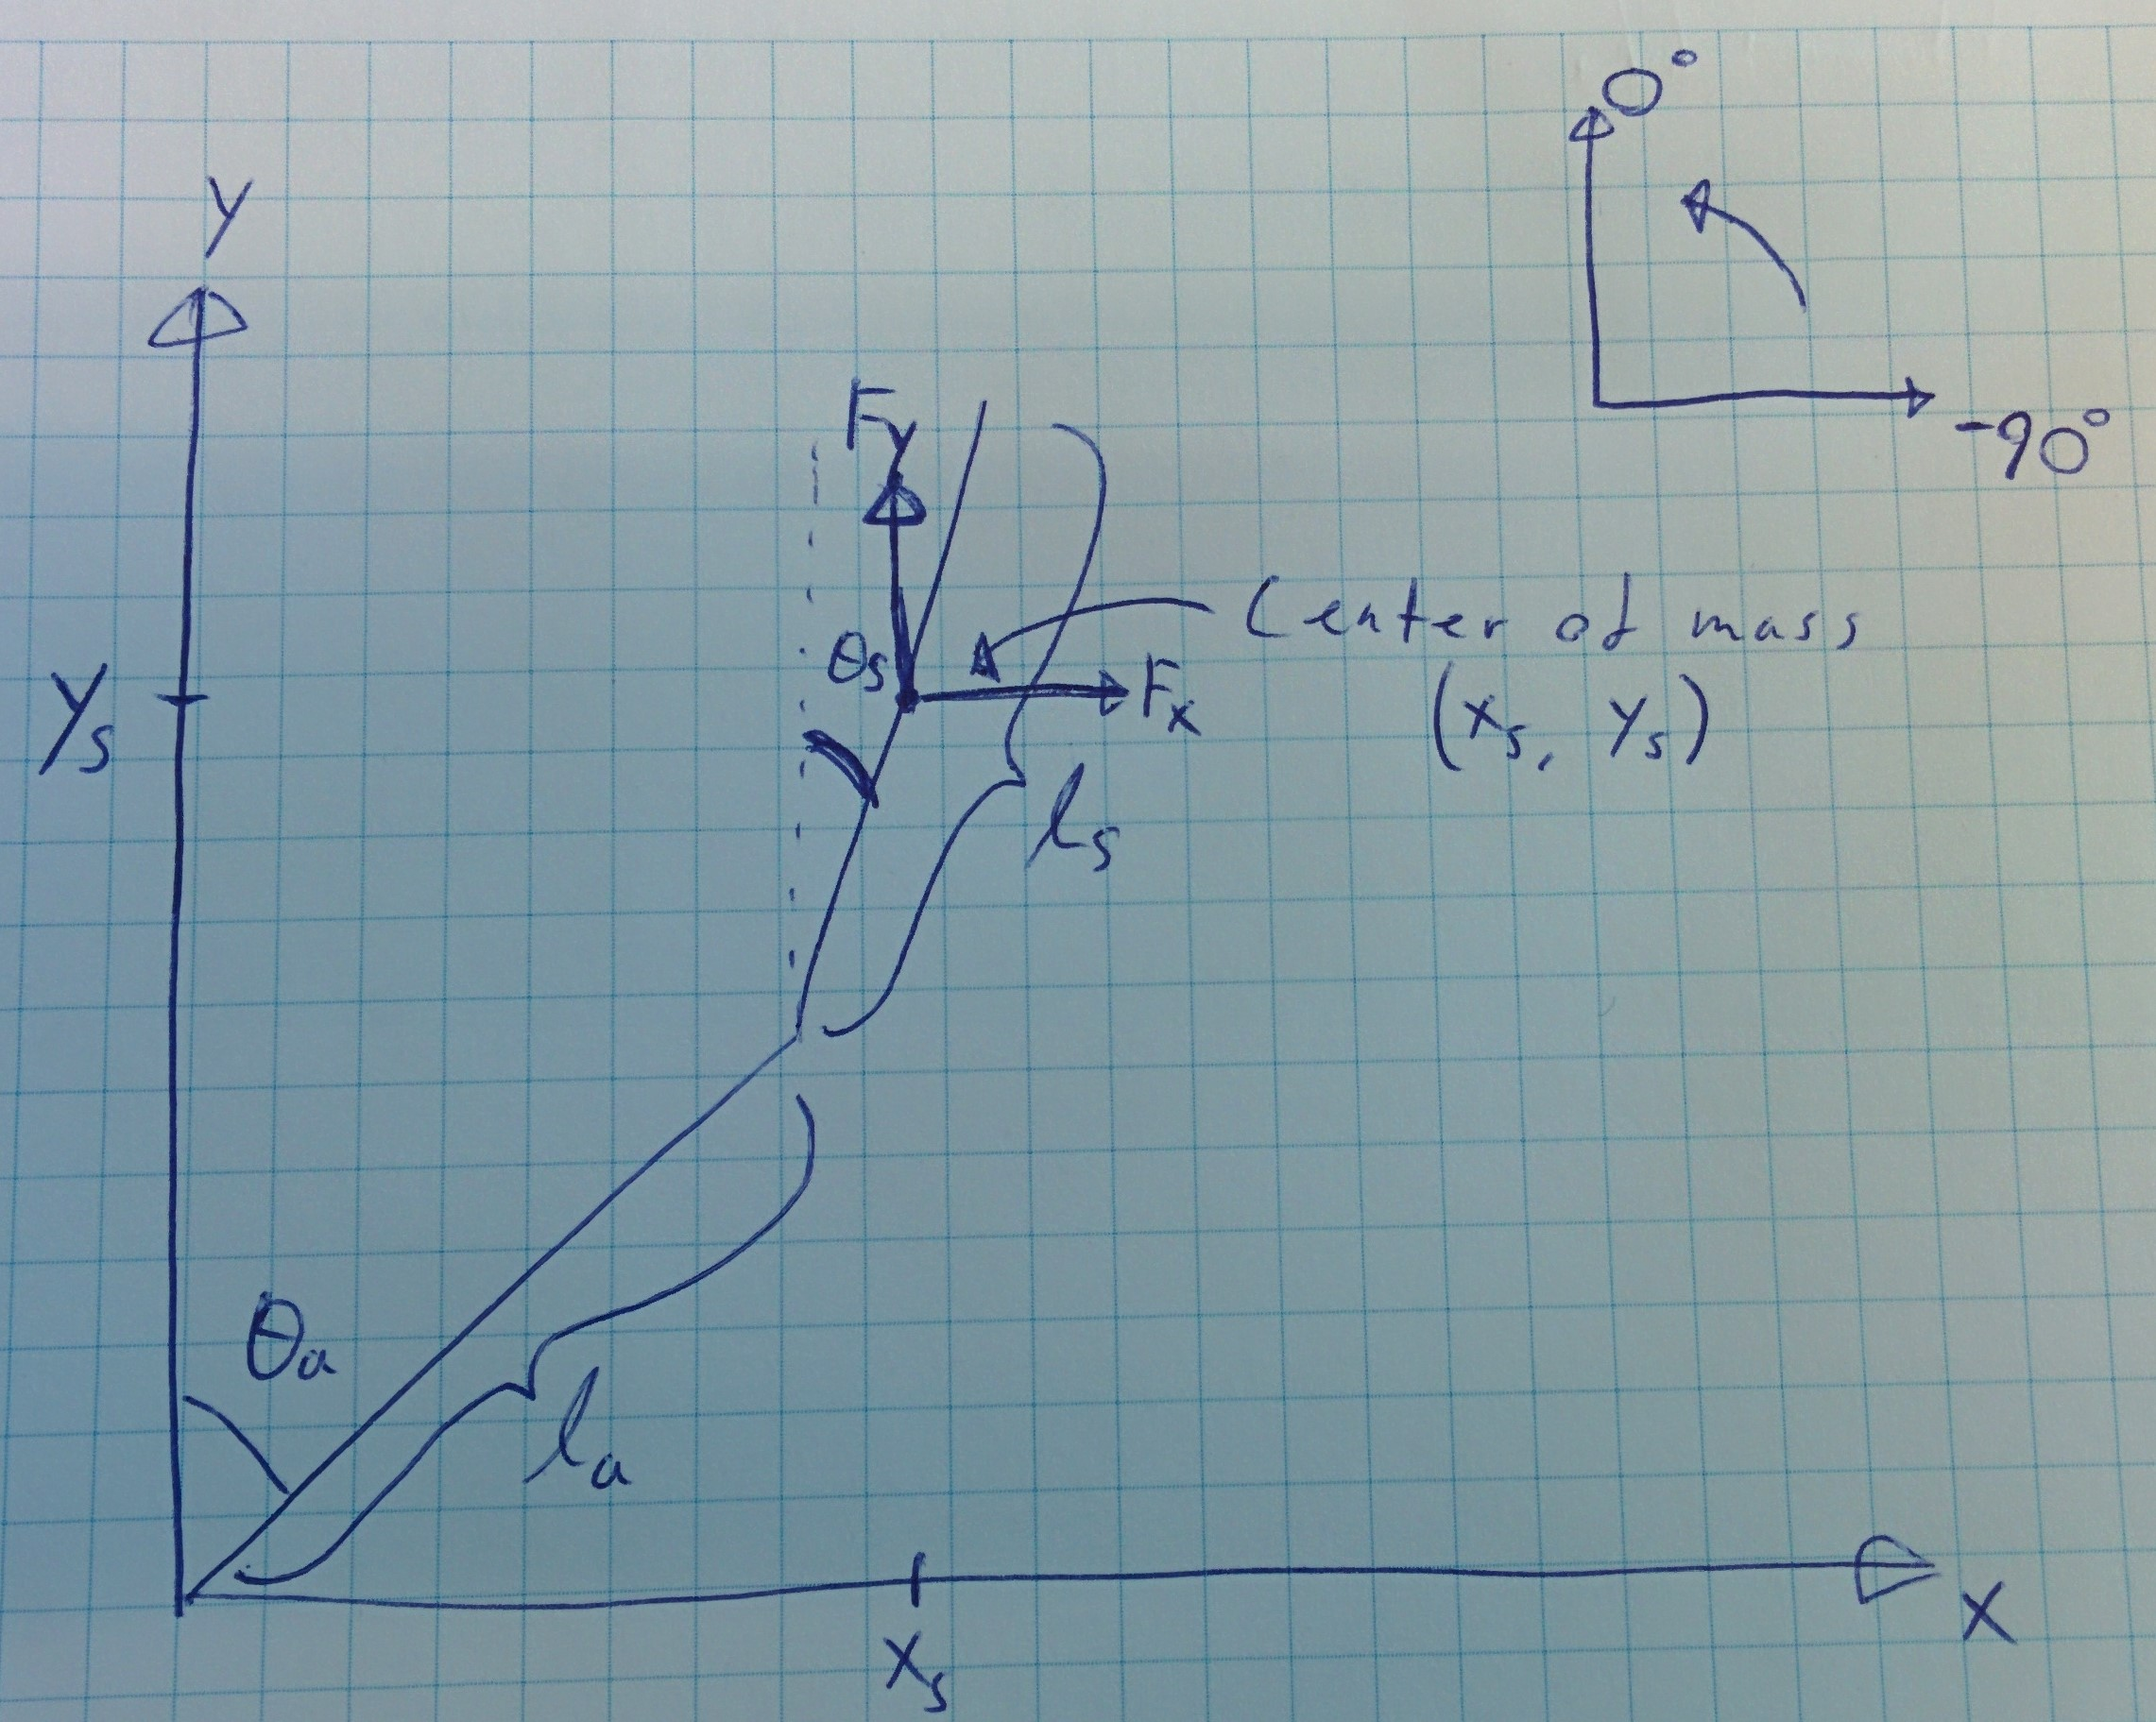
\includegraphics[width=0.8\textwidth]{StickAndForces}
\caption{Diagram of the angles and forces acting on the arm and the stick.}
\label{fig:ArmStick}
\end{figure}
\todo[inline,author=Jacob]{Make a pretty graph.}
All forces, constants and variables that relates to the arm and stick are denoted by a subscripted $a$ and $s$ respectively. 

To find the relation between the angles, the free body diagram of the joint of the arm and stick is made on \autoref{fig:freebodystick}.
\begin{figure}[htbp]
\centering
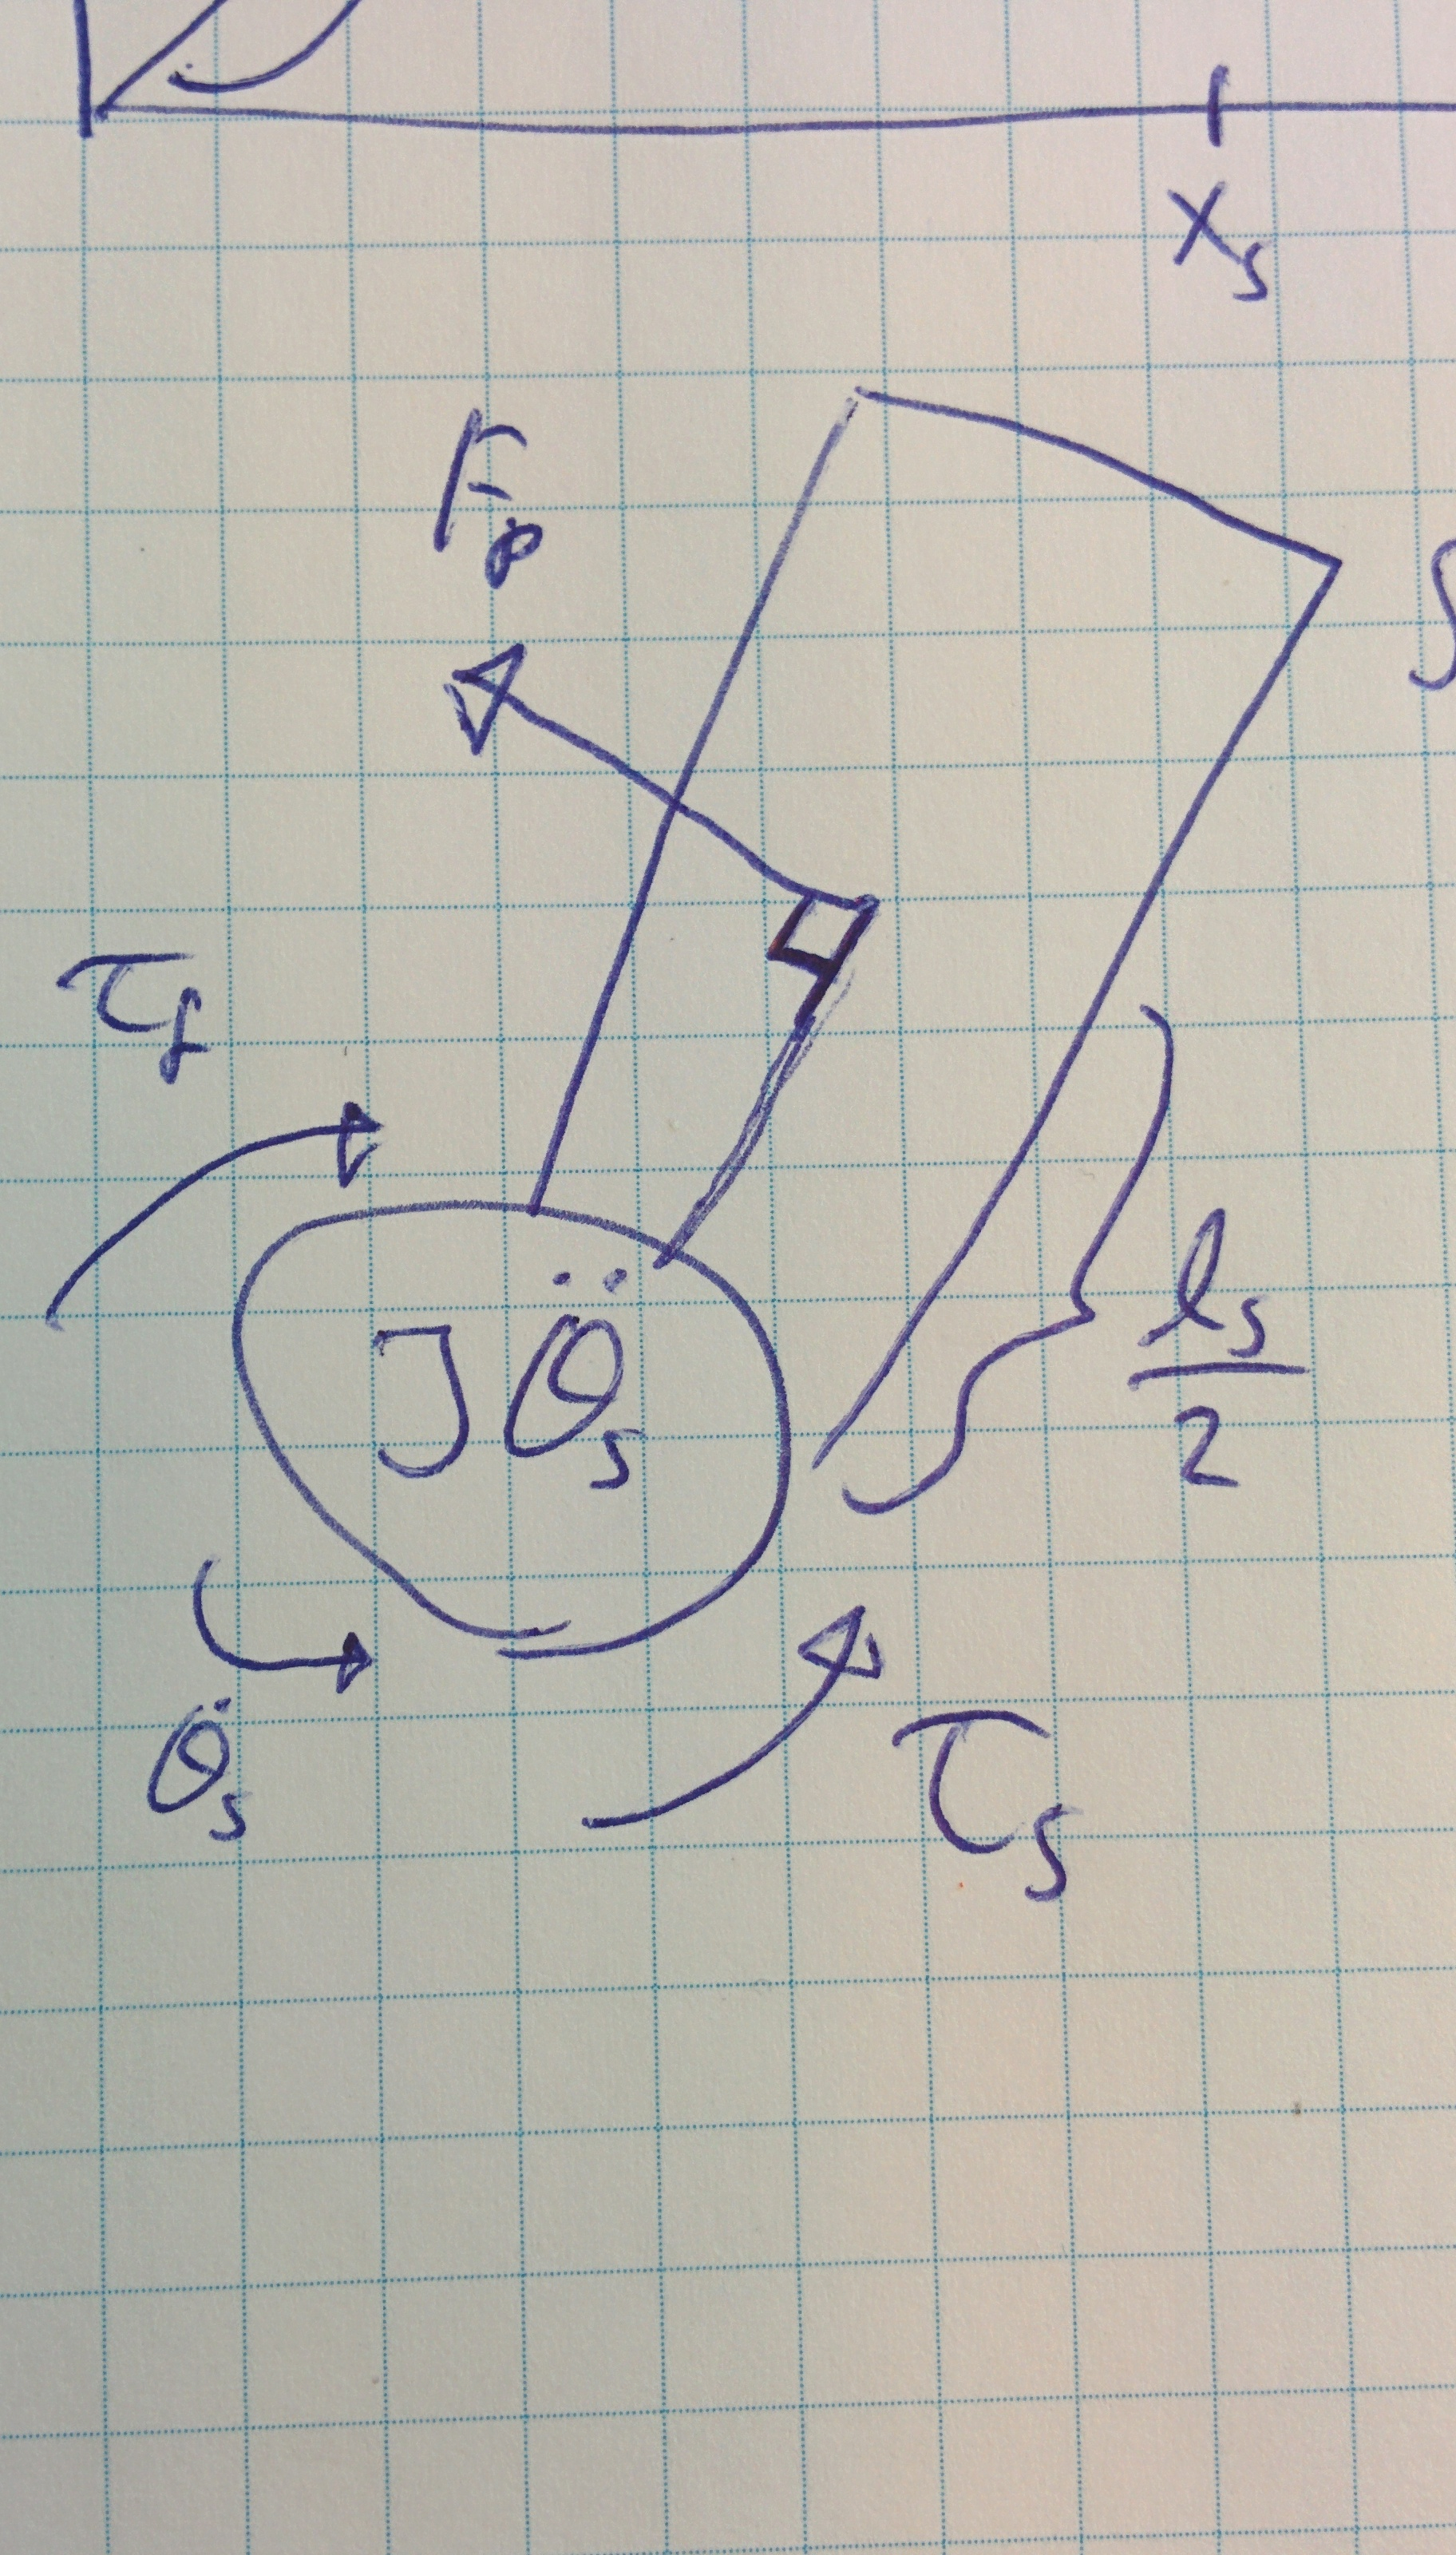
\includegraphics[width=0.25\textwidth]{FreeBodyPendulum}
\caption{Free body diagram of the joint that connects the arm and the stick.}
\label{fig:freebodystick}
\end{figure}
\todo[inline, author=Jacob]{Make pretty graph}

The moment of inertia for the joint is described by \autoref{eq:Jsthetas}.
\begin{subequations}
\begin{flalign}
& J_s\ddot{\theta}_s=\tau_s-\tau_f  \label{eq:Jsthetas} \\
& \tau_s =F_p\frac{l_s}{2} \\
& \tau_f =b_{as}\dot{\theta}_{as} 
\end{flalign}
\end{subequations}
\startexplain
	\explain{$J_s$ is the moment of inertia for the stick}{\si{\kg\square\meter}}
	\explain{$\tau_s$ is the torque induced by the rotation of the stick}{\si{\newton\meter}}
	\explain{$\tau_f$ is the torque of the friction acting on the stick}{\si{\newton\meter}}
	\explain{$F_p$ is the force perpendicular to the stick at the center of mass}{\si{\newton}}
	\explain{$b_{as}$ is the viscous friction coefficient between the arm and the stick}{\si{\newton\meter\second}}
	\explain{$\dot{\theta}_{as}$ is the difference in angular velocity between the arm and the stick}{\si{\degree\per\second}}
\stopexplain

The perpendicular force can be found from the forces acting on the stick in the x and y directions. These are found by \autoref{eq:FxFy} using Newton's 2nd law of motion.
\begin{subequations}  \label{eq:FxFy}
\begin{flalign}
	& F_x=\ddot{x}_sM_s  \\
	& F_y-gM_s=\ddot{y}_sM_s  \\
	& F_y=\left(\ddot{y}_s+g\right)M_s
\end{flalign}
\end{subequations}
\startexplain
	\explain{$F_x$ is the force in the x direction}{\si{\newton}}
	\explain{$F_y$ is the force in the y direction}{\si{\newton}}
	\explain{$x_s$ is the position of the center of mass of the stick in the x direction}{\si{\meter}}
	\explain{$y_s$ is the position of the center of mass of the stick in the y direction}{\si{\meter}}
	\explain{$M_s$ is the mass of the stick}{\si{\kilo\gram}}
\stopexplain
The position of the center of mass of the stick in the x and y direction is found by \autoref{eq:xsys}.
\begin{subequations}\label{eq:xsys} 
\begin{flalign}
& x_s=l_a\sin (-\theta_a)+\frac{l_s}{2} \sin (-\theta_s) \\
& x_s=-l_a\sin (\theta_a)-\frac{l_s}{2} \sin (\theta_s) \\
& y_s = l_a\cos (-\theta_a)+\frac{l_s}{2} \cos(-\theta_s) \\
& y_s = l_a\cos (\theta_a)+\frac{l_s}{2} \cos(\theta_s) 
\end{flalign}
\end{subequations}
\startexplain
	\explain{$l_a$ is the length of the arm}{\si{\meter}}
	\explain{$l_s$ is the length of the stick}{\si{\meter}}
	\explain{$\theta_a$ is the angle from the arm to the y-axis}{\si{\degree}}
	\explain{$\theta_s$ is the angle from the stick to the y-axis}{\si{\degree}}
\stopexplain
The derivatives of $x_s$ and $y_s$ is found in \autoref{eq:diffxy}.
\begin{subequations}\label{eq:diffxy} 
\begin{flalign}
\hspace{30pt} & \dot{x}_s=-l_a\dot{\theta}_a\cos(\theta_a)-\frac{l_s}{2}\dot{\theta}_s\cos(\theta_s) & [\si{\meter\per\second}] \\
& \ddot{x}_s=-l_a\ddot{\theta}_a\cos(\theta_a)+l_a\dot{\theta}_a^2\sin(\theta_a)-\frac{l_s}{2}\ddot{\theta}_s\cos(\theta_s)+\frac{l_s}{2}\dot{\theta}_s^2\sin(\theta_s) & [\si{\meter\per\square\second}] \\
& \dot{y}_s=-l_a \dot{\theta}_a\sin(\theta_a)-\frac{l_s}{2}\dot{\theta}_s\sin(\theta_s) & [\si{\meter\per\second}] \\
& \ddot{y}_s=-l_a\ddot{\theta}_a\sin(\theta_a)-l_a\dot{\theta}_a^2\cos(\theta_a)-\frac{l_s}{2}\ddot{\theta}_s\sin(\theta_s)-\frac{l_s}{2}\dot{\theta}_s^2\cos(\theta_s) & [\si{\meter\per\square\second}]
\end{flalign}
\end{subequations}

The forces $F_x$ and $F_y$ can be decomposed into perpendicular and parallel forces at that point. The parallel forces are negligible when assuming the stick is perfectly solid and unable to stretch or compress. The perpendicular forces is found by \autoref{eq:perpFxFy} and are seen on \autoref{fig:ForcePerp}.

\begin{figure}[htbp]
\centering
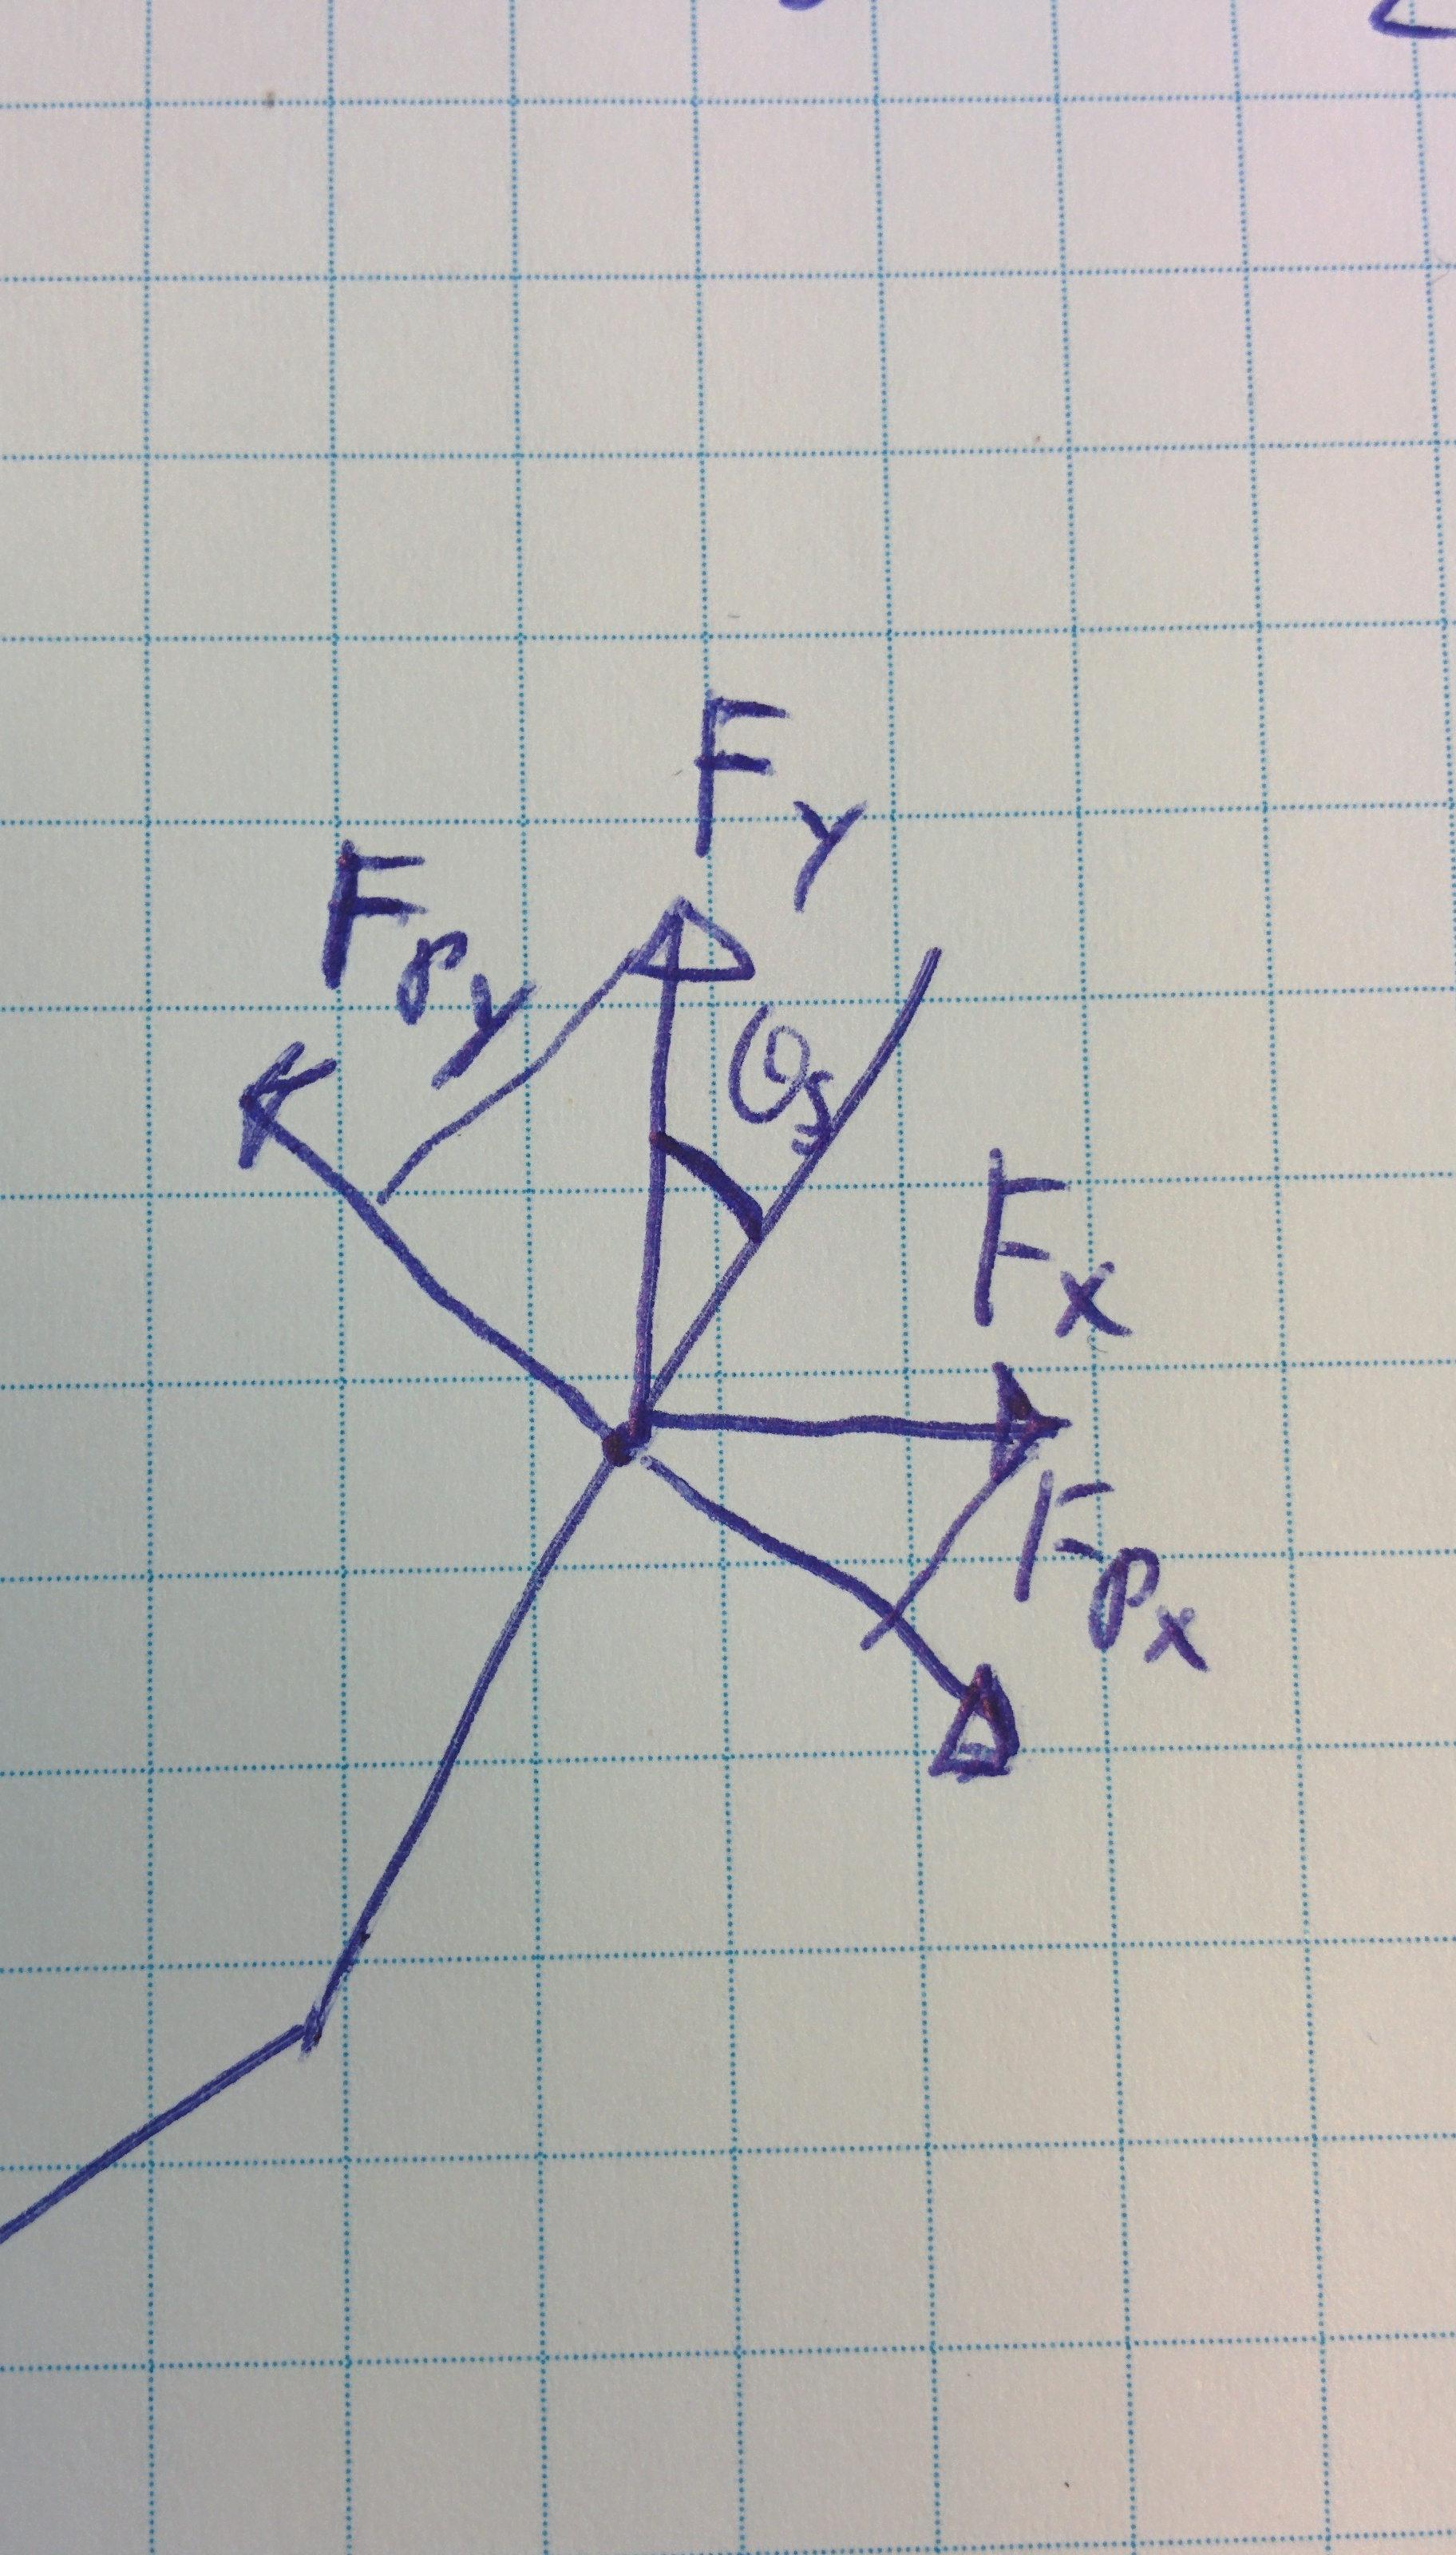
\includegraphics[width=0.25\textwidth]{ForcePerp}
\caption{Diagram of the forces, $F_x$ and $F_y$, decomposed into perpendicular forces.}
\label{fig:ForcePerp}
\end{figure}

\begin{subequations}\label{eq:perpFxFy}
\begin{flalign}
& F_{px}=F_x\cos(\theta_s) \\
& F_{py}=F_y\sin(\theta_s)  \\
& F_p = F_{px}+F_{py} 
\end{flalign}
\end{subequations}

Inserting $F_p$ into \autoref{eq:Jsthetas} gives \autoref{eq:JsLong}.
\begin{subequations}
\begin{flalign}
 J_s\ddot{\theta}_s &=\frac{l_s}{2}\left(F_x\cos(\theta_s)+F_y\sin(\theta_s)\right)-b_{as}\dot{\theta}_{as}  \\
 J_s\ddot{\theta}_s = \frac{l_s}{2}M_s \Big( &-l_a\ddot{\theta}_a\left(\cos(\theta_a)\cos(\theta_s)+\sin(\theta_a)\sin(\theta_s)\right) \notag \\
& +l_a\dot{\theta}_a^2\left(\sin(\theta_a)\cos(\theta_s)-\cos(\theta_a)\sin(\theta_s)\right) \notag \\
& -\frac{l_s}{2}\ddot{\theta}_s\left(\cos(\theta_s)\cos(\theta_s)+\sin(\theta_s)\sin(\theta_s)\right) \notag \\
& +\frac{l_s}{2}\dot{\theta}_s^2\left(\sin(\theta_s)\cos(\theta_s)-\cos(\theta_s)\sin(\theta_s)\right)  \notag \\
& +g\sin(\theta_s) \Big)-b_{as}\dot{\theta}_{as} \label{eq:JsLong}
\end{flalign}
\end{subequations}

Using the trigonometric properties in \autoref{eq:trigprop}, \autoref{eq:JsLong} is reduced to \autoref{eq:JsShort}.
\begin{subequations} \label{eq:trigprop}
\begin{flalign}
& \cos(\theta_a)\cos(\theta_s)\pm \sin(\theta_a)\sin(\theta_s)=\cos(\theta_a \mp \theta_s)  \\
& \sin(\theta_a)\cos(\theta_s)\pm \cos(\theta_a)\sin(\theta_s) = \sin(\theta_a \pm \theta_s) \\ 
& \cos(\theta_s)^2+\sin(\theta_s)^2=1 
\end{flalign}
\end{subequations}
\begin{flalign}
J_s\ddot{\theta}_s = \frac{l_s}{2}M_s \Big( &-l_a\ddot{\theta}_a \cos(\theta_a-\theta_s)+l_a\dot{\theta}_a^2 \sin(\theta_a-\theta_s) \notag \\
&-\frac{l_s}{2}\ddot{\theta}_s +g\sin(\theta_s) \Big)-b_{as}\dot{\theta}_{as} \label{eq:JsShort}
\end{flalign}

This is the nonlinear mathematical model for the system. This will be linearized in order to perform a Laplace transformation. The linearization is made with a 1st order Taylor approximation \textbf{[insert ref to note in google drive]}. The 1st order Taylor approximation of an equation with multiple variables is seen in \autoref{eq:1stTaylor}.
\begin{flalign}
 f\left(\theta_a, \dot{\theta}_a, \ddot{\theta}_a, \theta_s, \ddot{\theta}_s\right) & \approx f\left(\bar{\theta}_a, 0, 0, \bar{\theta}_s, 0\right) + \left. \frac{\partial f}{\partial \theta_a}\right|_{(\bar{\theta}_a, \bar{\theta}_s)} \hat{\theta}_a \notag \\
& \phantom{=} + \left. \frac{\partial f}{\partial \dot{\theta}_a}\right|_{(\bar{\theta}_a, \bar{\theta}_s)} \hat{\dot{\theta}}_a + \left. \frac{\partial f}{\partial \ddot{\theta}_a}\right|_{(\bar{\theta}_a, \bar{\theta}_s)} \hat{\ddot{\theta}}_a \notag \\
& \phantom{=} + \left. \frac{\partial f}{\partial \theta_s}\right|_{(\bar{\theta}_a, \bar{\theta}_s)} \hat{\theta}_s + \left. \frac{\partial f}{\partial \ddot{\theta}_s}\right|_{(\bar{\theta}_a, \bar{\theta}_s)} \hat{\ddot{\theta}}_s \label{eq:1stTaylor}
\end{flalign}
\startexplain
	\explain{$\bar{\theta}$ denotes the angle in an operating point}{\si{\degree}}
	\explain{$\hat{\theta}$ denotes the angle of the small signal variances}{\si{\degree}}
\stopexplain

The 3 terms with sin or cos in \autoref{eq:JsShort} will be approximated individually using \autoref{eq:1stTaylor}, remembering that $\bar{\theta}=\bar{\dot{\theta}}=\bar{\ddot{\theta}}=0$ as the angle of the operating point is a constant 0.
\begin{subequations}
\begin{flalign}
 -l_a\ddot{\theta}_a\cos\left(\theta_a-\theta_s\right) & \approx  0 + l_a\bar{\ddot{\theta}}_a\sin\left(\bar{\theta}_a-\bar{\theta}_s\right)\hat{\theta}_a  \notag \\ 
& \phantom{=} -l_a\cos\left(\bar{\theta}_a-\bar{\theta}_s\right)\hat{\ddot{\theta}}_a - l_a\bar{\ddot{\theta}}_a\sin\left(\bar{\theta}_a-\bar{\theta}_s\right)\hat{\theta}_s   \\
 -l_a\ddot{\theta}_a\cos\left(\theta_a-\theta_s\right) & \approx -l_a\hat{\ddot{\theta}}_a 
\end{flalign} %\bar{\ddot{\theta}}_s
\end{subequations}
\begin{subequations}
\begin{flalign}
l_a\dot{\theta}_a^2\sin\left(\theta_a-\theta_s\right) & \approx  0 + l_a\bar{\dot{\theta}}_a^2\cos\left(\bar{\theta}_a-\bar{\theta}_s\right)\hat{\theta}_a  \notag \\
& \phantom{=} + 2l_a\bar{\dot{\theta}}_a\sin\left(\bar{\theta}_a-\bar{\theta}_s\right)\hat{\dot{\theta}}_a-l_a\bar{\dot{\theta}}_a^2\cos\left(\bar{\theta}_a-\bar{\theta}_s\right)\hat{\theta}_s   \\
 l_a\dot{\theta}_a^2\sin\left(\bar{\theta}_a-\bar{\theta}_s\right) & \approx  0 
\end{flalign}
\end{subequations}
\begin{subequations}
\begin{flalign}
& g\sin\left(\theta_s\right) \approx g\sin\left(\bar{\theta}_s\right) +g\cos\left(\bar{\theta}_s\right)\hat{\theta}_s \\
& g\sin\left(\theta_s\right) \approx g\hat{\theta}_s 
\end{flalign}
\end{subequations}

Inserting the linearized terms in \autoref{eq:JsShort} and using the moment of inertia for a rotating stick, $J_s=\frac{1}{12}M_sl_s^2$, the linearized model becomes \eqref{eq:JsFinal}.
\begin{subequations}
\begin{flalign}
& \frac{1}{12}M_sl_s^2\hat{\ddot{\theta}}_s=\frac{l_s}{2}M_s\left(-l_a\hat{\ddot{\theta}}_a-\frac{l_s}{2}\hat{\ddot{\theta}}_s+g\hat{\theta}_s\right)-b_{as}\hat{\dot{\theta}}_{as}   \\
& \frac{1}{12}M_sl_s^2\hat{\ddot{\theta}}_s+\frac{1}{4}M_sl_s^2\hat{\ddot{\theta}}_s=\frac{l_s}{2}M_s\left(-l_a\hat{\ddot{\theta}}_a+g\hat{\theta}_s\right)-b_{as}\hat{\dot{\theta}}_{as}   \\
& \frac{1}{3}M_sl_s^2\hat{\ddot{\theta}}_s=\frac{l_s}{2}M_s\left(-l_a\hat{\ddot{\theta}}_a+g\hat{\theta}_s\right)-b_{as}\hat{\dot{\theta}}_{as}  \label{eq:TauSmLin} \\
& \hat{\ddot{\theta}}_s=\frac{3}{2l_s}\left(-l_a\hat{\ddot{\theta}}_a-\frac{l_s}{2}\hat{\ddot{\theta}}_s+g\hat{\theta}_s\right)-\frac{3b_{as}\left(\hat{\dot{\theta}}_s-\hat{\dot{\theta}}_a\right)}{M_sl_s^2} \label{eq:JsFinal}
\end{flalign}
\end{subequations}

The linearized model is now Laplace transformed in \autoref{eq:tfArmStick} in order to find the transfer function.
\begin{subequations}
\begin{flalign}
& s^2\Theta_s=\frac{3}{2l_s}\left(-s^2l_a\Theta_a+g\Theta_s\right)-s\frac{3b_{as}}{M_sl_s^2}\Theta_s+s\frac{3b_{as}}{M_sl_s^2}\Theta_a  \\
& \Theta_s\left(s^2+\frac{3b_{as}}{M_sl_s^2}s-\frac{3g}{2l_s}\right)=\Theta_a\left(-\frac{3l_a}{2l_s}s^2+\frac{3b_{as}}{M_sl_s^2}s\right)  \\
& \frac{\Theta_s}{\Theta_a}=-\frac{\frac{3l_a}{2l_s}s^2-\frac{3b_{as}}{M_sl_s^2}s}{s^2+\frac{3b_{as}}{M_sl_s^2}s-\frac{3g}{2l_s}} \label{eq:tfArmStick}
\end{flalign}
\end{subequations}

A linearized model in the Laplace domain for the arm and the stick has been derived and the model for the gears is now derived.
